\documentclass[12pt]{article}
\usepackage[a4paper, total={6in, 9in}]{geometry}
\usepackage[utf8]{inputenc}
\usepackage[polish]{babel}
\usepackage[T1]{fontenc}
\usepackage{lmodern}
\usepackage{minted}
\usepackage{tocloft}
\usepackage{titletoc}
\usepackage{secdot}
\usepackage{etoolbox}
\usepackage{graphicx}
\usepackage{hyperref}
\usepackage{amsmath}
\usepackage{wrapfig}
\usepackage{caption}
\usepackage{enumitem}
\usepackage{indentfirst}
\usepackage{chngcntr}
\usepackage{setspace}


\setlist[itemize]{itemsep=1pt, topsep=-5pt}
\setlist[enumerate]{itemsep=1pt, topsep=-5pt}

\title{Technologie obiektowe - projekt}
\author{Maciej Bandura, Marcin Ślusarczyk}

\begin{document}

\maketitle

\newpage
\include{Wstęp}
\section{Koncepcja mapowania obiektów na format CSV}

Opracowana została struktura pliku .csv, umożliwiająca efektywne mapowanie obiektów, do tego formatu. Pozwala ona na zapis wartości prymitywnych, list takich wartości, obiektów oraz list obiektów. Każdy zapisany obiekt, otrzymuje losowy identyfikator \mintinline{php}|uniqueid()|\footnote{https://www.php.net/manual/en/function.uniqid.php}, natomiast obiekty różnych klas zapisywane są w różnych plikach. Nazwy tych plików odpowiadają przestrzenią nazw tych klas w PHP. \\ \newline
W pierwszej linijce pliku .csv - nagłówku, przechowujemy informacje opisujące dane, są to, między innymi: nazwy pól w mappowanej klasie, wartości prefiksowane przy pomocy znaku "\textbf{\~}" informują nas o listach, natomiast wartości zawierające znak "\textbf{@}" wskazują na referencje do  obiektów (np. obiektów innej klasy). Dodatkowemu polu \textbf{id}, przypisano znak specjalny: "\textbf{\#}", tak aby nie kolidował z rzeczywistym polem \textit{id}, które często jest używane w obiektach. Znaki te zostały wybrane, ze względu na brak możliwości wystąpienia ich w rzeczywistej nazwie pola w języku PHP. Pozostała zawartość pliku csv nazywana przez nas \textit{ciałem}, zawiera rzeczywiste mapowanie do obiektów, opisane według definicji z nagłówka.

\paragraph{Przykład mappowania:} Klasa Student i Ocena 



\begin{figure}[ht]
	\centering
	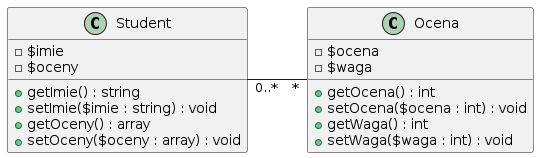
\includegraphics[width=0.8\textwidth]{materiały/st-oc}
	\caption{Mapowane klasy}
\end{figure}


\begin{empty}
	\begin{minted}[
		startinline,
		linenos,
		frame=lines,
		framesep=2mm,
		baselinestretch=1.2,
		fontsize=\footnotesize,
		breaklines,
		obeytabs=true,
		tabsize=2,
		]{text}
imie; ~oceny@TestListsObjs\Ocena; id#
Adam; 6664a3116c12c,6664a3116c131, ... ,6664a3116c13d; 6664a3116c124
	\end{minted}
	\vspace{-10pt}
	\captionof{listing}{Plik TestListsObjs-Student.csv}
\end{empty}
\vspace{10pt}
\begin{empty}
	\begin{minted}[
		startinline,
		linenos,
		frame=lines,
		framesep=2mm,
		baselinestretch=1.2,
		fontsize=\footnotesize,
		breaklines,
		obeytabs=true,
		tabsize=2,
		]{text}
ocena; waga; id#
6; 1; 6664a3116c12c
5; 2; 6664a3116c131
...
1; 6; 6664a3116c13d
	\end{minted}
	\vspace{-10pt}
	\captionof{listing}{Plik TestListsObjs-Ocena.csv}
\end{empty}

\section{Wykorzystanie}
Jak zostało wspomniane we wstępie, aby użyć mappera należy, wykorzystywać trait \mintinline{php}|CSVMapperInjector| oraz wywoływać pozyskaną metodę \mintinline{php}|injectDependencies()|.

\begin{empty}
	\begin{minted}[
		startinline,
		linenos,
		frame=lines,
		framesep=2mm,
		baselinestretch=1.2,
		fontsize=\footnotesize,
		breaklines,
		obeytabs=true,
		tabsize=2,
		]{php}
<?php
	require 'fake_vendor/autoload.php';
	require 'vendor/autoload.php';
	use CSVMapper\Boostrapper\CSVMapperInjector;
	
	class App 
	{
		use CSVMapperInjector;
		
		public function __construct ()
		{
			$this->injectDependencies();
		}
		
		/**
		* @CSVMapper
		*/
		private $csvMapper;
		
		public function main ()
		{
			var_dump($this->csvMapper);
		}
		
	}
	
	(new App())->main();
	\end{minted}
	\vspace{-10pt}
	\captionof{listing}{Przykład powołania mappera.}
\end{empty}

Mając już obiekt, \mintinline{php}|csvMappera|, możemy dokonywać operacji mapowania obiektów z pliku, jak i również ich zapisywania. Przy pomocy metod \mintinline{php}|read()| oraz \mintinline{php}|save()|.

\begin{empty}
	\begin{minted}[
		startinline,
		linenos,
		frame=lines,
		framesep=2mm,
		baselinestretch=1.2,
		fontsize=\footnotesize,
		breaklines,
		obeytabs=true,
		tabsize=2,
		]{php}
public function main ()
{
	$myClass = new MyClass();
	$this->csvMapper->save($myClass);
}
	\end{minted}
	\vspace{-10pt}
	\captionof{listing}{Przykład zapisu obiektu klasy \textbf{MyClass} do pliku.}
\end{empty}


\begin{empty}
	\begin{minted}[
		startinline,
		linenos,
		frame=lines,
		framesep=2mm,
		baselinestretch=1.2,
		fontsize=\footnotesize,
		breaklines,
		obeytabs=true,
		tabsize=2,
		]{php}
public function main ()
{
	$myObject = $this
		->csvMapper
		->read("./MyClass.csv", MyClass::class);
	
	var_dump($myObject);
}
	\end{minted}
	\vspace{-10pt}
	\captionof{listing}{Przykład odczytu obiektu klasy \textbf{MyClass} z pliku.}
\end{empty}
\section{Testy funkcjonalności}
W celu zachowania poprawności działania zostały przygotowane testy mające na celu sprawdzanie działania mappera. Testy opiewały o podstawowe funkcjonalności jak i te bardziej złożone. Za wykonywanie testów odpowiedzialny jest plik \mintinline{php}|tests.php|, zawiera on główną klasę \mintinline{php}|Tests|, która w konstruktorze powołuje konkretne testy rozszerzające klasę \mintinline{php}|Test|. Wszystkie testowane klasy zawierają metodę \mintinline{php}|test()|, w której zawarta jest logika testu. Metoda ta, musi zwrócić wartość wywołania  \mintinline{php}|pass()| - jeżeli test się powiedzie, lub \mintinline{php}|fail()| - jeżeli dojdzie to jakiegoś zdarzenia. Metody te odpowiednio obsłużą raportowanie wyników testu. 

\begin{figure}[ht]
	\centering
	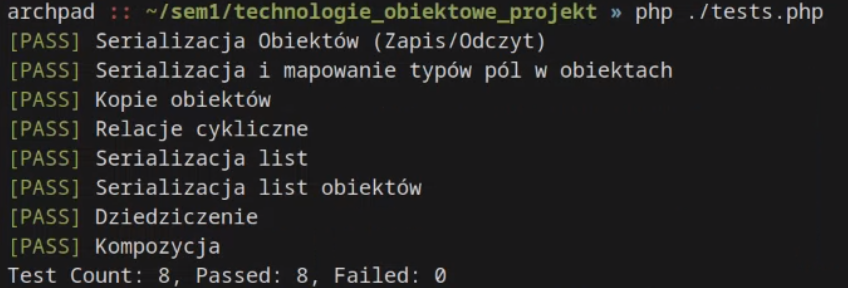
\includegraphics[width=0.9\textwidth]{materiały/raport}
	\caption{Raport wykonanych testów}
\end{figure}

\subsection{Test serializacji obiektów}
Jest to najbardziej podstawowy test, mają5cy na celu weryfikację działania mappera pod kątem zapisu i odczytu prostych obiektów, niezawierających list ani referencji do innych obiektów.

\begin{figure}[ht]
	\centering
	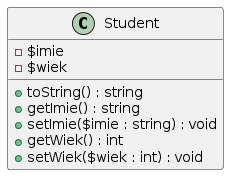
\includegraphics[width=0.3\textwidth]{materiały/student}
	\caption{Serializowana klasa \textbf{student}}
\end{figure}


\begin{empty}
	\begin{minted}[
		startinline,
		linenos,
		frame=lines,
		framesep=2mm,
		baselinestretch=1.2,
		fontsize=\footnotesize,
		breaklines,
		obeytabs=true,
		tabsize=2,
		]{text}
imie; wiek; id#
Tomek; 18; 666613345af2d
	\end{minted}
	\vspace{-10pt}
	\captionof{listing}{Wygenerowany plik TestSerializacjiObiektow-Student.csv}
\end{empty}


\begin{empty}
	\begin{minted}[
		startinline,
		linenos,
		frame=lines,
		framesep=2mm,
		baselinestretch=1.2,
		fontsize=\footnotesize,
		breaklines,
		obeytabs=true,
		tabsize=2,
		]{php}
public function test ()
{
	if ($this->mapper == null) {
		return $this->fail();
	}
	
	$student = new Student();
	$student->setWiek(18);
	$student->setImie("Tomek");
	
	$this->mapper->save($student);
	$fromFile = $this->mapper->read("./TestSerializacjiObiektow\Student.csv", Student::class);
	
	if (get_class($fromFile) != Student::class) {
		return $this->fail();
	}
	
	if ($student->toString() != $fromFile->toString()) {
		return $this->fail();
	}
	
	return $this->pass();
}
	\end{minted}
	\vspace{-10pt}
	\captionof{listing}{Logika testu.}
\end{empty}

\subsection{Test serializacji typów}
Kolejny, również prosty test, mający na celu sprawdzenie poprawności serializacji typów pól. Po zapisie sprawdzane jest, czy typy pól odczytanego obiektu zgadzają się z typami oryginalnego obiektu. 

\begin{empty}
	\begin{minted}[
		startinline,
		linenos,
		frame=lines,
		framesep=2mm,
		baselinestretch=1.2,
		fontsize=\footnotesize,
		breaklines,
		obeytabs=true,
		tabsize=2,
		]{php}
if (gettype($fromFile->getWysokosc()) != gettype($student->getWysokosc())) {
	return $this->fail();
}
if (gettype($fromFile->getWiek()) != gettype($student->getWiek())) {
	return $this->fail();
}
if (gettype($fromFile->getImie()) != gettype($student->getImie())) {
	return $this->fail();
}
	\end{minted}
	\vspace{-10pt}
	\captionof{listing}{Logika testu.}
\end{empty}

\subsection{Test kopii obiektów}
Test ma na celu zweryfikować, poprawność serializacji wielu referencji do tego samego obiektu, w obiekcie \textbf{A}, pola \mintinline{php}|$b1|  oraz \mintinline{php}|$b2| zawierają referencje do tego samego obiektu. Natomiast pole \mintinline{php}|$b3| zawiera referencje do innego obiektu tej samej klasy. Test upewnia się, że zostaną zserializowane tylko dwie instancje klasy \textbf{B}, oraz to, że zostaną one poprawnie zmapowane po odczytaniu.  

\begin{figure}[ht]
	\centering
	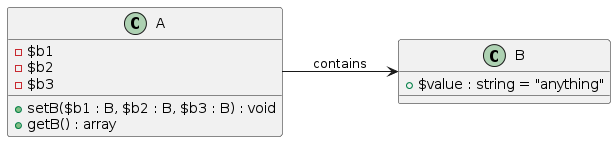
\includegraphics[width=0.75\textwidth]{materiały/kopie}
	\caption{Serializowane klasy}
\end{figure}

\begin{empty}
	\begin{minted}[
		startinline,
		linenos,
		frame=lines,
		framesep=2mm,
		baselinestretch=1.2,
		fontsize=\footnotesize,
		breaklines,
		obeytabs=true,
		tabsize=2,
		]{text}
b1@TestObjectCopies\B; b2@TestObjectCopies\B; b3@TestObjectCopies\B; id#
666619324645f; 666619324645f; 6666193246466; 6666193246459
	\end{minted}
	\vspace{-10pt}
	\captionof{listing}{Plik TestObjectCopies-A.csv}
\end{empty}


\begin{empty}
	\begin{minted}[
		startinline,
		linenos,
		frame=lines,
		framesep=2mm,
		baselinestretch=1.2,
		fontsize=\footnotesize,
		breaklines,
		obeytabs=true,
		tabsize=2,
		]{text}
value; id#
anything; 666619324645f
anything; 6666193246466
	\end{minted}
	\vspace{-10pt}
	\captionof{listing}{Plik TestObjectCopies-B.csv}
\end{empty}

\subsection{Test serializacji list}
Prosty test serializacji list typów prymitywnych. 

\begin{figure}[ht]
	\centering
	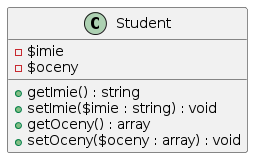
\includegraphics[width=0.35\textwidth]{materiały/sam_student}
	\caption{Mapowana klasa}
\end{figure}

\begin{empty}
	\begin{minted}[
		startinline,
		linenos,
		frame=lines,
		framesep=2mm,
		baselinestretch=1.2,
		fontsize=\footnotesize,
		breaklines,
		obeytabs=true,
		tabsize=2,
		]{text}
imie; ~oceny; id#
Szymek; 2,2,3,1; 66661932466e6
	\end{minted}
	\vspace{-10pt}
	\captionof{listing}{Plik TestLists-Student.csv}
\end{empty}

\subsection{Test serializacji list obiektów}
Jest to rozszerzenie poprzedniego testu o referencje do obiektów innej klasy. Idea testu pozostaje taka sama.

\begin{figure}[ht]
	\centering
	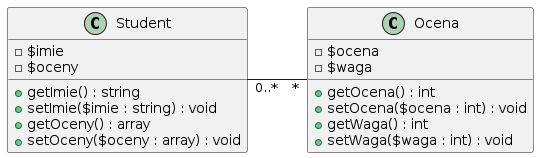
\includegraphics[width=0.7\textwidth]{materiały/st-oc}
	\caption{Mapowana klasa}
\end{figure}

Struktura plików .csv została zaprezentowana we wstępie. 


\subsection{Test - dziedziczenie}
W programowaniu obiektowym jednym z podstawowych narzędzie jest dziedziczenie oraz implementowanie. Oczywistym jest, że nasz mapper musi współpracować z obiektami posługującymi się tymi narzędziami. Test ten ma na celu weryfikację, czy odtworzony obiekt odpowiednio dziedziczy po klasie \mintinline{php}|Osoba| oraz czy implementuje interfejs \mintinline{php}|Witalny|.

\begin{figure}[ht]
	\centering
	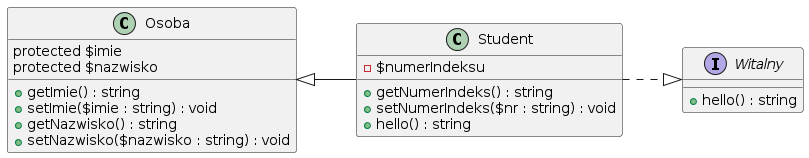
\includegraphics[width=0.82\textwidth]{materiały/dziedziczenie}
	\caption{Mapowana klasa}
\end{figure}

\begin{empty}
	\begin{minted}[
		startinline,
		linenos,
		frame=lines,
		framesep=2mm,
		baselinestretch=1.2,
		fontsize=\footnotesize,
		breaklines,
		obeytabs=true,
		tabsize=2,
		]{php}
if (!($fromFile instanceof Student)) {
	return $this->fail();
}

if (!($fromFile instanceof Osoba)) {
	return $this->fail();
}

if (!($fromFile instanceof Witalny)) {
	return $this->fail();
}
	\end{minted}
	\vspace{-10pt}
	\captionof{listing}{Logika testu}
\end{empty}

\begin{empty}
	\begin{minted}[
		startinline,
		linenos,
		frame=lines,
		framesep=2mm,
		baselinestretch=1.2,
		fontsize=\footnotesize,
		breaklines,
		obeytabs=true,
		tabsize=2,
		]{text}
		numerIndeksu; imie; nazwisko; id#
		abc123; Kamil; Ślimak; 6666193246903
	\end{minted}
	\vspace{-10pt}
	\captionof{listing}{Plik TestDziedziczenia-Student.csv}
\end{empty}


\subsection{Test - kompozycja}
Kolejnym narzędziem wykorzystywanym w technologiach obiektowych jest kompozycja. Poniższy test, zapewnia, pełną obsługę kompozycji przez naszego mappera. 

\begin{figure}[ht]
	\centering
	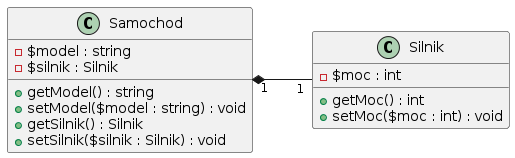
\includegraphics[width=0.7\textwidth]{materiały/kompozycja2}
	\caption{Mapowana klasa}
\end{figure}

\begin{empty}
	\begin{minted}[
		startinline,
		linenos,
		frame=lines,
		framesep=2mm,
		baselinestretch=1.2,
		fontsize=\footnotesize,
		breaklines,
		obeytabs=true,
		tabsize=2,
		]{php}
if ($fromFile->getModel() != $bmw->getModel()) {
	return $this->fail();
}

if (!($fromFile->getSilnik() instanceof Silnik)) {
	return $this->fail();
}

if ($fromFile->getSilnik()->getMoc() != $silnik->getMoc()) {
	return $this->fail();
}
	\end{minted}
	\vspace{-10pt}
	\captionof{listing}{Logika testu}
\end{empty}

\begin{empty}
	\begin{minted}[
		startinline,
		linenos,
		frame=lines,
		framesep=2mm,
		baselinestretch=1.2,
		fontsize=\footnotesize,
		breaklines,
		obeytabs=true,
		tabsize=2,
		]{text}
model; silnik@TestKompozycja\Silnik; id#
528i; 66661932469af; 66661932469a8
	\end{minted}
	\vspace{-10pt}
	\captionof{listing}{Plik TestKompozycja-Samochod.csv}
\end{empty}

\begin{empty}
	\begin{minted}[
		startinline,
		linenos,
		frame=lines,
		framesep=2mm,
		baselinestretch=1.2,
		fontsize=\footnotesize,
		breaklines,
		obeytabs=true,
		tabsize=2,
		]{text}
moc; id#
245KM; 66661932469af
	\end{minted}
	\vspace{-10pt}
	\captionof{listing}{Plik TestKompozycja-Silnik.csv}
\end{empty}

\subsection{Test relacji cyklicznych}
Relacje cykliczne zwane również rekurencyjnymi są ciekawym zjawiskiem, do których często dochodzi przez przypadek w środowiskach produkcyjnych. Niezależnie od tego, czy są dobrymi praktykami, czy nie, nasz mapper musi je wspierać. Ważne jest aby w trakcie odtwarzania obiektów, nie dopuścić do zapętlenia mappera. Takie zjawisko można wykryć przy pomocy tego testu. 

\begin{figure}[ht]
	\centering
	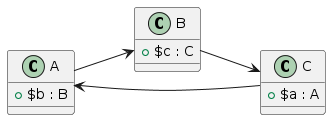
\includegraphics[width=0.5\textwidth]{materiały/relacje}
	\caption{Mapowana klasa}
\end{figure}

\begin{empty}
	\begin{minted}[
		startinline,
		linenos,
		frame=lines,
		framesep=2mm,
		baselinestretch=1.2,
		fontsize=\footnotesize,
		breaklines,
		obeytabs=true,
		tabsize=2,
		]{php}
if ($fromFile->b->c->a !== $fromFile) {
	return $this->fail();
}
	\end{minted}
	\vspace{-10pt}
	\captionof{listing}{Logika testu}
\end{empty}

\section{Mappery na inne formaty}
\paragraph{}Jak zostało wspomniane we wstępie, nasz mapper jest w stanie obsługiwać różne formaty, nie tylko .csv. Nie mniej jednak nie posiada on logiki do dokładnego mapowania z każdego z obsługiwanych formatów. Posiada on serię konwerterów między formatowych pozwalających tłumaczyć różne formaty na csv i na odwrót. Mechanizm działania samego mappera współpracuje tylko i wyłącznie z formatem csv, konwertery zapewniają dodatkową warstwę wsparcia poszerzając wachlarz wspieranych formatów. Konwersja ta, realizowana jest przy pomocy mechaniki \mintinline{php}|ExtensionProvider|, gdzie każdy konkretny "\textit{dostawca rozszerzeń}" funkcjonuje jako swojego rodzaju tłumacz między rdzeniem mappera a konkretnymi formatami.

\begin{figure}[ht]
	\centering
	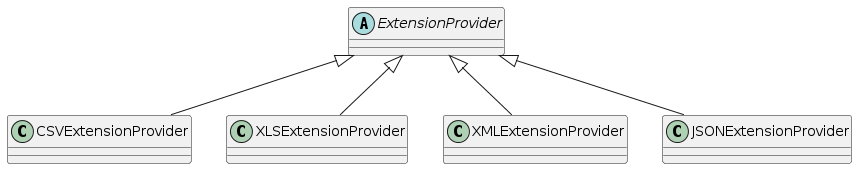
\includegraphics[width=1.0\textwidth]{materiały/hierarchia}
	\caption{Dostępni dostawcy formatów/rozszerzeń}
\end{figure}

Konkretnego dostawcę możemy wstrzyknąć do instancji mappera, przy pomocy metody \mintinline{php}|provideExtension(ExtensionProvider)|, nadpisując w ten sposób domyślnego dostawcę, tj. \mintinline{php}|CSVExtensionProvider|.

\begin{empty}
	\begin{minted}[
		startinline,
		linenos,
		frame=lines,
		framesep=2mm,
		baselinestretch=1.2,
		fontsize=\footnotesize,
		breaklines,
		obeytabs=true,
		tabsize=2,
		]{php}
public function main ()
{
	$this->csvMapper
	->provideExtension(new XMLExtensionProvider())
	->save($this->a);
	
	$x = $this->csvMapper
	->read("./A.csv", A::class);
}
	\end{minted}
	\vspace{-10pt}
	\captionof{listing}{Wstrzyknięcie dostawcy formatu XML}
\end{empty}

\paragraph{Uwaga:} Mimo, że jako ścieżkę podaliśmy plik z rozszerzeniem \textit{.csv}, to dostawca doklei do niego rozszerzenie \textit{.xml}.

\newpage
\subsection{CSVExtensionProvider}
Jest to domyślny oraz najprostszy dostawca, którego zadaniem jest tylko zapisać i odczytać podany plik. 

\begin{empty}
	\begin{minted}[
		startinline,
		linenos,
		frame=lines,
		framesep=2mm,
		baselinestretch=1.2,
		fontsize=\footnotesize,
		breaklines,
		obeytabs=true,
		tabsize=2,
		]{php}
namespace CSVMapper\ExtensionProvider;
use CSVMapper\ExtensionProvider\ExtensionProvider;

class CSVExtensionProvider implements ExtensionProvider
{
	public function write ($file, $csv)
	{
		file_put_contents($file, $csv);
	}
	
	public function read ($file)
	{
		return file_get_contents($file);
	}
}
	\end{minted}
	\vspace{-10pt}
	\captionof{listing}{CSVExtensionProvider}
\end{empty}

\subsection{XMLExtensionProvider}
Nieco bardziej zaawansowanym dostawcą jest, ten od formatu XML. Wykorzystując wbudowaną w język PHP bibliotekę \mintinline{php}|DOMDocument|, odpowiednio tworzy i parsuje pliki .xml na podstawie dostarczanych danych w formacie CSV.

\begin{empty}
	\begin{minted}[
		startinline,
		linenos,
		frame=lines,
		framesep=2mm,
		baselinestretch=1.2,
		fontsize=\footnotesize,
		breaklines,
		obeytabs=true,
		tabsize=2,
		]{xml}
<?xml version="1.0"?>
<Mapping>
	<Definition>
		<Field>moc</Field>
		<Field>id#</Field>
	</Definition>
	<Content>
		<Entity>
			<Value>245KM</Value>
			<Value> 66662740bf785</Value>
		</Entity>
	</Content>
</Mapping>
	\end{minted}
	\vspace{-10pt}
	\captionof{listing}{TestKompozycja-Silnik.csv.xml}
\end{empty}

\begin{empty}
	\begin{minted}[
		startinline,
		linenos,
		frame=lines,
		framesep=2mm,
		baselinestretch=1.2,
		fontsize=\footnotesize,
		breaklines,
		obeytabs=true,
		tabsize=2,
		]{xml}
<?xml version="1.0"?>
<Mapping>
	<Definition>
		<Field>model</Field>
		<Field> silnik@TestKompozycja\Silnik</Field>
		<Field>id#</Field>
	</Definition>
	<Content>
		<Entity>
			<Value>528i</Value>
			<Value> 66662740bf785</Value>
			<Value> 66662740bf77f</Value>
		</Entity>
	</Content>
</Mapping>
	\end{minted}
	\vspace{-10pt}
	\captionof{listing}{TestKompozycja-Samochod.csv.xml}
\end{empty}

\begin{empty}
	\begin{minted}[
		startinline,
		linenos,
		frame=lines,
		framesep=2mm,
		baselinestretch=1.2,
		fontsize=\footnotesize,
		breaklines,
		obeytabs=true,
		tabsize=2,
		]{php}
public function write ($file, $csv)
{
	$lines = explode("\n", $csv);
	$header = explode(";", array_shift($lines));
	
	$domDoc = new DOMDocument;
	$root = $domDoc->createElement('Mapping');
	...
	foreach ($header as $tok) {
		/**
		* Konwersja nagłowka ...
		*/
	}
	
	$content = $domDoc->createElement('Content');
	$root->appendChild($content);
	foreach ($lines as $line) {
		/**
		* Konwersja ciała ...
		*/
	}
	
	file_put_contents($file . ".xml", $domDoc->saveXML());
}
	\end{minted}
	\vspace{-10pt}
	\captionof{listing}{Fragment metody zapisu}
\end{empty}

\subsection{JSONExtensionProvider}
JSON jest jednym z najbardziej popularnych formatów, wymiany danych. Język PHP zawiera wbudowane funkcje do obsługi tego formatu, dlatego też, stworzenie konwertera nie stanowiło dużego wyzwania. 

\begin{empty}
	\begin{minted}[
		startinline,
		linenos,
		frame=lines,
		framesep=2mm,
		baselinestretch=1.2,
		fontsize=\footnotesize,
		breaklines,
		obeytabs=true,
		tabsize=2,
		]{php}
public function read ($file)
{
	$json = file_get_contents($file . ".json");
	$root = json_decode($json);
	
	$header = [];
	$entities = [];
	
	$first = (array) $root->entities[0];
	foreach ($first as $key => $value) {
		$header[] = $key;
	}
	
	foreach ($root->entities as $entity) {
		$values = [];
		foreach ((array) $entity as $value) {
			$values[] = $value;
		}
		$entities[] = implode(";", $values);
	}
	
	return implode(";", $header) . "\n" . implode("\n", $entities);
}
	\end{minted}
	\vspace{-10pt}
	\captionof{listing}{Metoda odczytu}
\end{empty}

\begin{empty}
	\begin{minted}[
		startinline,
		linenos,
		frame=lines,
		framesep=2mm,
		baselinestretch=1.2,
		fontsize=\footnotesize,
		breaklines,
		obeytabs=true,
		tabsize=2,
		]{json}
{
	"entities":[
		{
			"model":"528i",
			" silnik@TestKompozycja\\Silnik":" 666629a031291",
			" id#":" 666629a031289"
		}
	]
}
	\end{minted}
	\vspace{-10pt}
	\captionof{listing}{TestKompozycja-Samochod.csv.json}
\end{empty}

\begin{empty}
	\begin{minted}[
		startinline,
		linenos,
		frame=lines,
		framesep=2mm,
		baselinestretch=1.2,
		fontsize=\footnotesize,
		breaklines,
		obeytabs=true,
		tabsize=2,
		]{json}
{
	"entities":[
		{
			"moc":"245KM",
			" id#":" 666629a031291"
		}
	]
}
	\end{minted}
	\vspace{-10pt}
	\captionof{listing}{TestKompozycja-Silnik.csv.json}
\end{empty}

\begin{empty}
	\begin{minted}[
		startinline,
		linenos,
		frame=lines,
		framesep=2mm,
		baselinestretch=1.2,
		fontsize=\footnotesize,
		breaklines,
		obeytabs=true,
		tabsize=2,
		]{php}
		public function write ($file, $csv)
		{
			$lines = explode("\n", $csv);
			$header = explode(";", array_shift($lines));
			
			$root = (object) ["entities" => []];
			
			foreach ($lines as $line) {
				$toks = explode(";", $line);
				$newObj = [];
				for ($i = 0; $i < count($toks); $i++) {
					$newObj[$header[$i]] = $toks[$i];
				}
				$root->entities[] = (object) $newObj;
			}
			
			file_put_contents($file . ".json", json_encode($root));
		}
	\end{minted}
	\vspace{-10pt}
	\captionof{listing}{Metoda zapisu}
\end{empty}

\subsection{XLSExtensionProvider}
Ostatnim z obsługiwanych formatów jest XLS. W przypadku poprzednich formatów każdy rodzaj klasy był zapisany w osobnym pliku. W tym przypadku zostało zastosowane inne podejście - obiekty tych samych klas zapisywane są we wspólnych \textit{arkuszach}. Takie podejście wiąże się, z dodatkowymi komplikacjami. Format XLS posiada rygorystyczne ograniczenia dotyczące nazw arkuszy, dlatego też wszystkie nazwy musimy haszować, tak aby spełniały one wspomniane kryteria. Dodatkowym problemem jest maksymalna długość nazwy, a mianowicie, jest to 31 znaków. Funkcja haszująca z której korzystamy, do zabezpieczania nazw, to \mintinline{php}|md5()|, problem leży w tym, że funkcja ta, produkuje hasze o długości 32 znaków. Został on rozwiązany poprzez odcięcie ostatniego znaku. Ponieważ, osoba analizująca arkusz, własnoręcznie może mieć problemy z transkrypcją haszy na nazwy plików, do każdego zmapowanego pliku \textit{.xlsx}, dołączamy dodatkowy arkusz zawierający indeks nazw i odpowiadających im haszy. Ponadto język PHP natywnie nie wspiera formatu XLS, wymagana jest instalacja dodatkowej biblioteki \mintinline{php}|phpoffice/phpspreadsheet|. Aby tego dokonać, należy użyć narzędzia \textbf{composer} wywołując poniższe polecenie:\\
\mintinline{text}|# composer require phpoffice/phpspreadsheet|\\
Biblioteka ta, dodatkowo może wymagać konfiguracji ustawień samego PHP. Należy upewnić się, że poniższe moduły są włączone:\\
\mintinline{text}|extension=gd|\\
\mintinline{text}|extension=iconv|\\

\begin{figure}[ht]
	\centering
	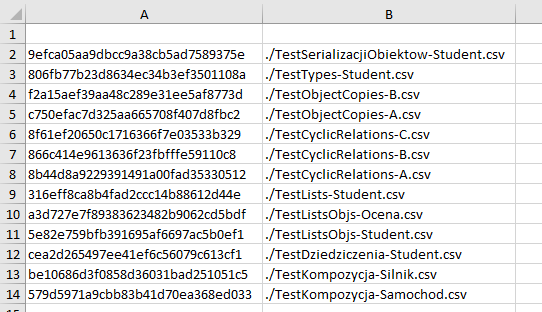
\includegraphics[width=0.9\textwidth]{materiały/excel1}
	\caption{Indeks nazw arkuszy}
\end{figure}

\begin{figure}[ht]
	\centering
	
\includegraphics[width=1.0\textwidth]{materiały/excel2}
	\caption{Widok dostępnych arkuszy w pliku}
\end{figure}

\begin{figure}[ht]
	\centering
	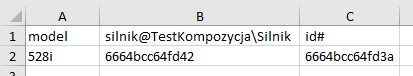
\includegraphics[width=0.7\textwidth]{materiały/excel3}
	\caption{Arkusz TestKompozycja-Samochod.csv}
\end{figure}
\section{Wykorzystane wzorce projektowe}
\subsection{Strategia}
Wzorzec projektowy strategia to behawioralny wzorzec projektowy, który umożliwia definiowanie rodziny algorytmów, enkapsulowanie każdego z nich oraz uczynienie ich wymienialnymi. Wzorzec ten pozwala na zmienianie algorytmów niezależnie od klientów, które z nich korzystają. Główne elementy wzorca Strategia to: Kontekst (Context), Strategia (Strategy) oraz Konkretne Strategie (Concrete Strategies). Kontekst to klasa, która zawiera referencję do obiektu Strategii i deleguje do niego wykonanie pewnych operacji. Strategia to interfejs wspólny dla wszystkich algorytmów, który definiuje metodę, jaką muszą implementować wszystkie konkretne strategie. Konkretne Strategie to klasy implementujące interfejs Strategii, zawierające konkretne algorytmy. Wzorzec Strategia jest użyteczny, gdy istnieje potrzeba dynamicznego wyboru algorytmu w trakcie działania programu lub gdy chcemy uniknąć umieszczania wielu złożonych warunków w kodzie. Dzięki temu wzorcowi kod staje się bardziej elastyczny i łatwiejszy do utrzymania.

W przypadku naszego projektu, użyliśmy tego wzorca do implementacji dostawców formatów (konwerterów)
\begin{figure}[ht]
	\centering
	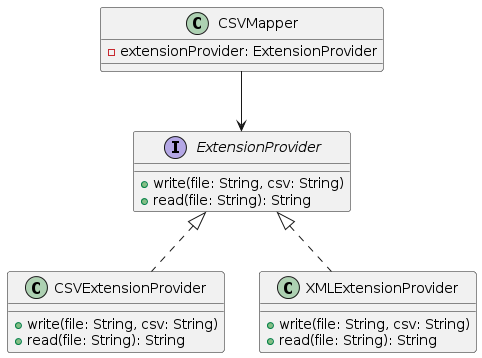
\includegraphics[width=0.65\textwidth]{materiały/strategia}
	\caption{Wykorzystanie strategii}
\end{figure}

\subsection{Iterator}
Iterator to behawioralny wzorzec projektowy, który umożliwia sekwencyjne przechodzenie przez elementy kolekcji bez ujawniania jej wewnętrznej struktury (takiej jak lista, stos, drzewo, itp.). Dzięki temu wzorcowi można uzyskać jednolity interfejs do przeglądania różnych typów kolekcji, co ułatwia manipulację i przetwarzanie danych. Główne elementy wzorca Iterator to: Iterator, Kolekcja (Collection) oraz Konkretne Iteratory (Concrete Iterators). Iterator to interfejs definiujący metody do iterowania po elementach kolekcji, takie jak hasNext() (sprawdzająca, czy są jeszcze elementy do przejścia) oraz next() (zwracająca kolejny element). Konkretne Iteratory to klasy implementujące interfejs Iteratora, które zawierają logikę potrzebną do przechodzenia po konkretnej strukturze danych.

\paragraph{} W przypadku naszego projektu, użyliśmy tego wzorca do implementacji wykrywania adnotacji w klasach wykorzystujących mappera.

\begin{figure}[ht]
	\centering
	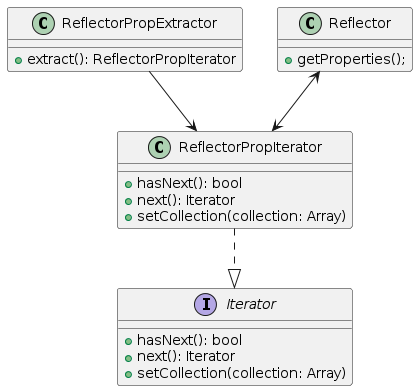
\includegraphics[width=0.55\textwidth]{materiały/iterator}
	\caption{Wykorzystanie iteratora}
\end{figure}


\subsection{Dekoratror}
Dekorator to strukturalny wzorzec projektowy, który pozwala dynamicznie dodawać nowe obowiązki obiektom poprzez umieszczanie tych obiektów w specjalnych obiektach opakowujących, które zawierają odpowiednie zachowania. Dzięki temu wzorcowi można rozszerzać funkcjonalność obiektów bez modyfikowania ich kodu bazowego. W kontekście PHP, dekorator może być również implementowany za pomocą cech (traits). Traits w PHP to mechanizm pozwalający na wielokrotne wykorzystanie kodu w różnych klasach.

\begin{figure}[ht]
	\centering
	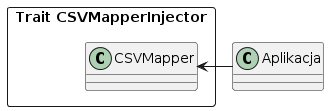
\includegraphics[width=0.4\textwidth]{materiały/dekorator}
	\caption{Wykorzystanie dekoratora}
\end{figure} 
\section{Podsumowanie}
Projekt można uznać za ukończony. Wszystkie założone funkcjonalności zostały zaprojektowanie i zaimplementowane. Mapper sprostał coraz to nowym wymaganiom stawianym w trakcie trwania semestru. Testy były ważnym narzędziem w trakcie prac nad projektem, nie tylko sprawdzały poprawność wprowadzanych funkcjonalności, ale również nakreślały drogę rozwoju projektu. Dlatego też złożoność testów jest różna, od tych prostszych po te bardziej zaawansowane.

Projekt współpracuje z wieloma formatami, gdzie każdy z nich został sprawdzony przy pomocy przedstawionego zestawu testów. Obsługę wielu formatów można było rozwiązać na dwa główne sposoby:
\paragraph{Pierwszy:} dla każdego formatu można było stworzyć dedykowany mapper, wymagałoby to znacznych zmian w istniejącym kodzie. Tak naprawdę to należałoby rozdzielić istniejącą mechanikę na dwie, obsługę plików \textit{.csv} oraz klasę do zarządzania mapowaniem ogólnie. Wiązałoby się to z bardzo dużym nakładem pracy, natomiast sam projekt znacznie odstawałby od swojej pierworodnej idei. 
\paragraph{Drugi:} można było stworzyć mechanizm konwerterów, współpracujący, z już gotową mechaniką mappera CSV - tak jak to zostało robione. Zastosowane podejście, zdało test, ma ono swoje plusy ale również minusy.
\paragraph{Plusy:}
\begin{itemize}
	\item Stosunkowo mała ilość zmian w istniejącym kodzie.
	\item Bardzo szybki development nowych dostawców formatów.
	\item Rozdzielona odpowiedzialność między konwerterami a mapperem.
	\item Nie ogranicza nas abstrakcja danych w formacie, z perspektywy mappera.
\end{itemize}

\paragraph{Minusy:}
\begin{itemize}
	\item Niska wydajność w porównaniu do dedykowanego mappera konkretnego formatu
	\item Wszelkie niedociągnięcia następujące w trakcie konwersji.
\end{itemize}





\end{document}
